% !BIB program = biber 
\documentclass{article}

%----------------------------------------------------------------------------------------
%	PACKAGES AND OTHER DOCUMENT CONFIGURATIONS
%----------------------------------------------------------------------------------------

% Generate dummy text (lorem ipsum) in your document
\usepackage{lipsum} % Comment me

% English language hyphenation
\usepackage[english]{babel}

% Math packages
\usepackage{amsmath, amsfonts, amsthm}

% Indent first paragraph
\usepackage{indentfirst}

% Figures
\usepackage{float}
\usepackage{graphicx}
\graphicspath{{./images/}}

% Captions
\usepackage{caption}
\usepackage{subcaption}

% Context sensitive quotation facilities
\usepackage{csquotes}

% Enumerate
\usepackage{enumitem}

% Chemical formulas package
\usepackage{chemformula}

% Filesystem
\usepackage{forest}

% Minted package for syntax highlighting
\usepackage{minted}

% Table 
\usepackage[toc]{appendix}
\addto\captionsenglish{% Replace "english" with the language you use
  \renewcommand{\contentsname}{Table of Contents}
}

% Shorthands
\usepackage{xspace}
\makeatletter
\DeclareRobustCommand\onedot{\futurelet\@let@token\@onedot}
\def\@onedot{\ifx\@let@token.\else.\null\fi\xspace}

\def\eg{e.g\onedot} \def\Eg{E.g\onedot}
\def\ie{i.e\onedot} \def\Ie{I.e\onedot}
\def\cf{cf\onedot} \def\Cf{Cf\onedot}
\def\etc{etc\onedot} \def\vs{vs\onedot}
\def\wrt{w.r.t\onedot} \def\dof{d.o.f\onedot}
\def\etal{et al.\onedot}
\makeatother

% Hyperlinks styling
\usepackage{hyperref}
% Hyperlink setup
\hypersetup{
  colorlinks   = true, % Colours links instead of ugly boxes
  urlcolor     = blue, % Colour for external hyperlinks
  linkcolor    = blue, % Colour of internal links
  citecolor    = blue, % Colour of citations
  linktocpage  = true, % Link only on page numbers
}
% PDF metadata
\hypersetup{
  pdftitle     = {Guia do usuário: Co-localização de parasitas de Chagas em
      células musculares cardíacas},
  pdfauthor    = {Patrick. H. F. Alvares, João V. S. Guerra, José G. C.
      Pereira},
  pdfproducer  = {Latex with hyperref},
  pdfcreator   = {pdflatex}
}

% Bibliography
\usepackage[
  backend=biber,
  style=ieee,
  natbib=true,
]{biblatex}
\addbibresource{\jobname.bib}

% Acronyms
\usepackage[
  printonlyused,
  nohyperlinks,
  withpage,
]{acronym}

%----------------------------------------------------------------------------------------
%	DOCUMENT MARGINS
%----------------------------------------------------------------------------------------

\usepackage{geometry} % Required for adjusting page dimensions and margins
\geometry{
  paper=a4paper,
  top=30mm, % Top margin
  bottom=20mm, % Bottom margin
  left=30mm, % Left margin
  right=20mm, % Right margin
  % showframe, % Uncomment to show how the type block is set on the page
}

%----------------------------------------------------------------------------------------
%	FONTS
%----------------------------------------------------------------------------------------

% Required for inputting international characters
\usepackage[T1]{fontenc}
% Use 8-bit encoding
\usepackage[latin1,utf8]{inputenc}

% Fonts
\usepackage{lmodern}

% Title Page
\long\def\reporttitle{%
  \begin{titlepage}
    % Logo
    \begin{center}
      \begin{minipage}{0.9\textwidth}%

        
\includegraphics[width=\textwidth]{lnbio-cnpem-logo.png}%
      \end{minipage}
    \end{center}
    \vskip 1em

    % Horizontal line
    \hline
    \vskip 2em

      % Title
      {\centering \LARGE Guia do usuário: Co-localização de parasitas de
        Chagas em células musculares cardíacas \par}
    \vskip 2em

      % Author
      {\centering \large Patrick. H. F. Alvares, João V. S. Guerra, José G.
        C. Pereira \par} % CHANGE
    \vskip 2em

      % Date
      {\centering \large \today\par}
    \vskip 1em

    % Horizontal line
    \hline

    % Do not break page
    \let\endtitlepage\relax
  \end{titlepage}
  
  % Version
  \vfill
  {\centering v1.0.0\par}
}

\begin{document}

% Make title
\reporttitle
\break

% Table of Contents
\hline
\tableofcontents
\vskip 0.5em
\hline
\break 

\section{Introdução}

Este guia do usuário fornece instruções detalhadas sobre como executar a análise de co-localização de parasitas de Chagas em células musculares cardíacas. O objetivo deste guia é auxiliar os usuários a configurar e executar o pipeline de análise, bem como a interpretar os resultados obtidos.

\section{Requisitos}

Para executar a análise de co-localização de parasitas de Chagas em células musculares cardíacas, você precisará dos seguintes requisitos:

\begin{itemize}
  \item \textbf{Acesso ao GitHub do CNPEM}: Você deve ter acesso ao repositório do projeto (\url{https://github.com/cnpem/ParasiteCoLocalization}) no GitHub do CNPEM (\url{https://github.com/cnpem/}) para baixar os arquivos necessários. Se não tiver acesso, entre em contato com a Equipe de Dados Biológicos (\url{edb@lnbio.cnpem.br}).
  \item \textbf{Acesso ao HPCC Marvin}: Você deve ter acesso ao HPCC Marvin para executar o pipeline de análise. Se você não tiver acesso, acesse \url{https://marvindocs.cnpem.br/primeiros-passos/index.html}.
\end{itemize}

\section{Acessando o HPCC Marvin}

Para acessar o HPCC Marvin, comece abrindo o terminal. Se estiver usando Windows, abra o PowerShell; se estiver usando Linux ou MacOS, abra o Terminal. Para acessar o HPCC Marvin, use o comando:

\begin{minted}[frame=single, bgcolor=lightgray, fontsize=\small]{bash}
ssh <seu.login.cnpem>@marvin.cnpem.br
\end{minted}

Após inserir o comando, será solicitado que você insira sua senha, digite sua senha institucional.

\section{Preparando o Repositório \texttt{ParasiteCoLocalization}}

Para clonar o repositório \href{https://github.com/cnpem/ParasiteCoLocalization}{ParasiteCoLocalization}, execute o seguinte comando no terminal:

\begin{minted}[frame=single, bgcolor=lightgray, fontsize=\small]{bash}
git clone https://github.com/cnpem/ParasiteCoLocalization.git
\end{minted}

O comando acima cria uma pasta chamada \texttt{ParasiteCoLocalization} no diretório atual. Esta pasta contém todos os arquivos necessários para a execução da análise de co-localização de parasitas de Chagas em células musculares cardíacas, incluindo o script \texttt{run.sh}, que automatiza a execução da análise via SLURM.

Após clonar o repositório \texttt{ParasiteCoLocalization}, acesse o diretório do projeto com o comando:

\begin{minted}[frame=single, bgcolor=lightgray, fontsize=\small]{bash}
cd ParasiteCoLocalization
\end{minted}

\subsection{Instalando PyEnv no HPCC Marvin}

O PyEnv é uma ferramenta que permite instalar e gerenciar várias versões do Python em um ambiente virtual. Para instalar o PyEnv no HPCC Marvin, execute os seguintes comandos no terminal:

\begin{minted}[frame=single, bgcolor=lightgray, fontsize=\small]{bash}
curl https://pyenv.run | bash
echo 'export PATH="$HOME/.pyenv/bin:$PATH"' >> ~/.bashrc
echo 'eval "$(pyenv init -)"' >> ~/.bashrc
echo 'eval "$(pyenv virtualenv-init -)"' >> ~/.bashrc
source ~/.bashrc
\end{minted}

Para instalar uma versão específica do Python, execute o seguinte comando:

\begin{minted}[frame=single, bgcolor=lightgray, fontsize=\small]{bash}
pyenv install 3.8.19
\end{minted}

Para definir a versão do Python como padrão neste diretório, execute o seguinte comando:

\begin{minted}[frame=single, bgcolor=lightgray, fontsize=\small]{bash}
pyenv local 3.8.19
\end{minted}

Caso deseje utilizar outra versão do Python, você pode selecionar a versão desejada para a sessão atual com o comando:

\begin{minted}[frame=single, bgcolor=lightgray, fontsize=\small]{bash}
pyenv shell <versão_desejada>
\end{minted}

\subsection{Instalando as Dependências do Python}

Para instalar as dependências do Python, execute o seguinte comando no terminal:

\begin{minted}[frame=single, bgcolor=lightgray, fontsize=\small]{bash}
pip install -r requirements.txt
\end{minted}

\subsection{Enviando Imagens para o HPCC Marvin}

Para enviar as imagens para o HPCC Marvin, você pode usar o comando \texttt{scp} em qualquer terminal.

\begin{minted}[frame=single, bgcolor=lightgray, fontsize=\small, breaklines]{bash}
scp /caminho/para/suas/imagens/*.tiff <seu.login.cnpem>@marvin.cnpem.br:/caminho/para/ParasiteCoLocalization/data
\end{minted}

Caso você esteja usando o Windows, você pode usar o \href{WinSCP}{https://winscp.net/eng/download.php} para transferir arquivos de e para o HPCC Marvin. Para isso, siga as instruções abaixo:

\begin{enumerate}
  \item Abra o WinSCP e insira o endereço do servidor (\texttt{marvin.cnpem.br}), seu nome de usuário e senha.
  \item Navegue até o diretório \texttt{ParasiteCoLocalization/data} no HPCC Marvin.
  \item Arraste e solte os arquivos de imagem do seu computador para o diretório \texttt{ParasiteCoLocalization/data} no HPCC Marvin.
\end{enumerate}

\subsection{Executando o Pipeline no HPCC Marvin}

Após enviar as imagens para o HPCC Marvin, você pode executar o pipeline de análise de co-localização de parasitas de Chagas em células musculares cardíacas. O script \texttt{run.sh} executa o pipeline de análise via SLURM, que é o sistema de gerenciamento de tarefas usado no HPCC Marvin. Para isso, execute o script \texttt{run.sh} no diretório \texttt{ParasiteCoLocalization}.

\begin{minted}[frame=single, bgcolor=lightgray, fontsize=\small]{bash}
cd ParasiteCoLocalization
sbatch run.sh -m marvin
\end{minted}

O comando acima retorna o ID do job SLURM, que você pode usar para monitorar o progresso da análise.

\subsubsection{Monitoramento do Job SLURM}

Para monitorar o progresso do job SLURM, você pode usar o comando \texttt{squeue} no terminal. O comando \texttt{squeue} exibe informações sobre os jobs SLURM em execução no HPCC Marvin.

\begin{minted}[frame=single, bgcolor=lightgray, fontsize=\small]{bash}
squeue -u <seu.login.cnpem>
\end{minted}

Se o job estiver em execução, o estado será exibido como R (em execução). Se o job estiver aguardando na fila, o estado será PD (pendente).

Caso deseje cancelar o job SLURM, você pode usar o comando \texttt{scancel} no terminal. O comando \texttt{scancel} cancela um job SLURM em execução no HPCC Marvin.

\begin{minted}[frame=single, bgcolor=lightgray, fontsize=\small]{bash}
scancel <job_id>
\end{minted}

Por fim, você pode verificar o arquivo de log gerado pelo SLURM (\texttt{slurm\_<job\_id>.out}) para obter informações sobre o seu job.

\section{Visualizando os Resultados}

Após a conclusão da análise, os resultados serão armazenados no diretório \texttt{results/}, que incluem os seguintes arquivos:

\begin{itemize}
  \item \texttt{summary.csv}: Este arquivo contém um resumo dos resultados da análise por poço, incluindo contagem total de células, contagem total de parasitas, contagem de células infectadas ($>3$ parasitas), taxa de infecção, e número mediano de parasitas por célula.

\begin{minted}[frame=single, bgcolor=lightgray, fontsize=\footnotesize]{markdown}
|     | TotalCells | TotalSpots | InfectedCells | InfectionRate      | MedianSpotsPerInfectedCell |
| --- | ---------- | ---------- | ------------- | ------------------ | -------------------------- |
| A1  | 726.0      | 5993.0     | 155           | 21.349862258953166 | 23.0                       |
| A2  | 593.0      | 5176.0     | 165           | 27.82462057335582  | 16.0                       |
| A3  | 759.0      | 7076.0     | 232           | 30.566534914361    | 18.0                       |
| A4  | 679.0      | 6243.0     | 170           | 25.03681885125184  | 23.0                       |
| A5  | 601.0      | 5898.0     | 164           | 27.287853577371045 | 19.5                       |
| A6  | 715.0      | 6112.0     | 187           | 26.153846153846157 | 18.0                       |
| A7  | 551.0      | 4285.0     | 172           | 31.21597096188748  | 13.0                       |
| A8  | 625.0      | 5036.0     | 161           | 25.759999999999998 | 17.0                       |
\end{minted}
  
  \item \texttt{plate\_map/}: Este diretório contêm os mapas interativos da placa de 384 poços (Figura \ref{fig:plate_map}), contendo:

  \begin{itemize}
    \item \texttt{number\_of\_cells.html}: contagem total de células por poço.
    \item \texttt{number\_of\_spots.html}: contagem total de parasitas por poço.
    \item \texttt{median\_spots\_per\_infected\_cell.html}: número mediano de parasitas por célula por poço.
    \item \texttt{infection\_rate.html}: razão entre o número de células infectadas e o número total de células por poço.
  \end{itemize}

  \begin{figure}[H]
    \centering
    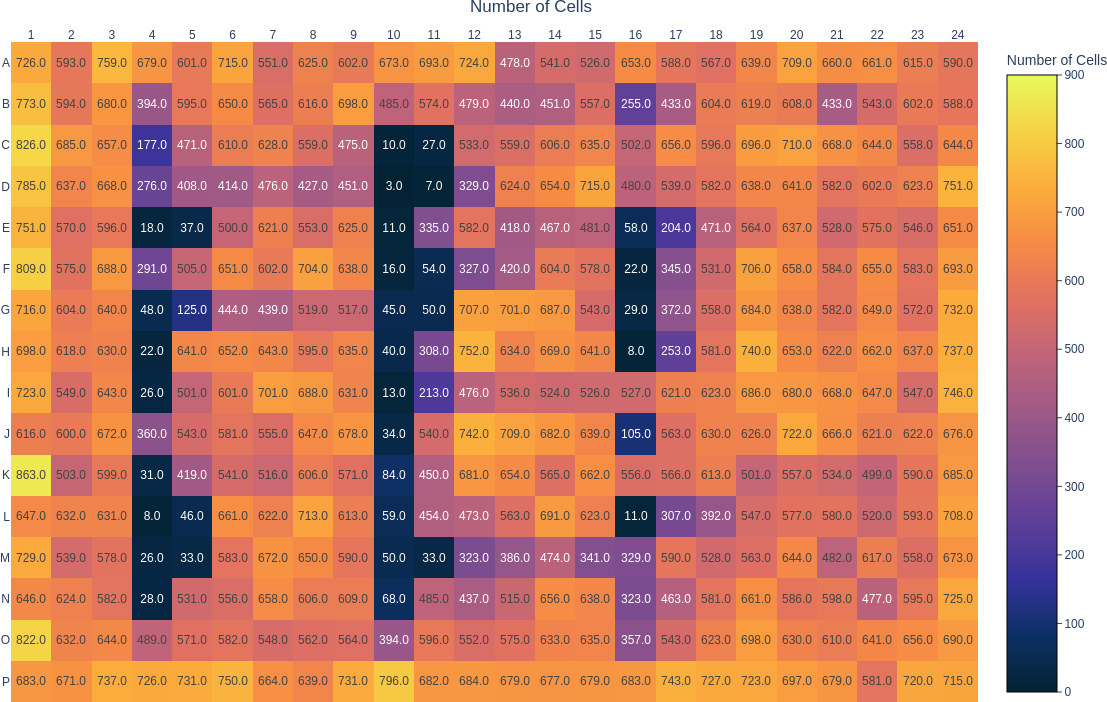
\includegraphics[width=0.65\textwidth]{images/example_plate_map.png}
    \caption{Exemplo de mapa interativo da placa de 384 poços.}
    \label{fig:plate_map}
  \end{figure}

  \item \texttt{scatter/}: Este diretório contêm os gráficos de dispersão interativos para a placa de 384 poços (Figura \ref{fig:scatter}), contendo:
  
  \begin{itemize}
    \item \texttt{number\_of\_cells\_vs\_number\_of\_infected\_cells.html}: relação entre o número de células e o número de células infectadas.
    \item \texttt{number\_of\_cells\_vs\_infection\_rate.html}: relação entre o número de células e a taxa de infecção.
    \item \texttt{median\_spots\_per\_infected\_cell\_vs\_number\_of\_cells.html}: relação entre o número mediano de parasitas por célula infectada e o número de células.
    \item \texttt{median\_spots\_per\_infected\_cell\_vs\_infection\_rate.html}: relação entre o número mediano de parasitas por célula infectada e a taxa de infecção.
  \end{itemize}

  \begin{figure}[H]
    \centering
    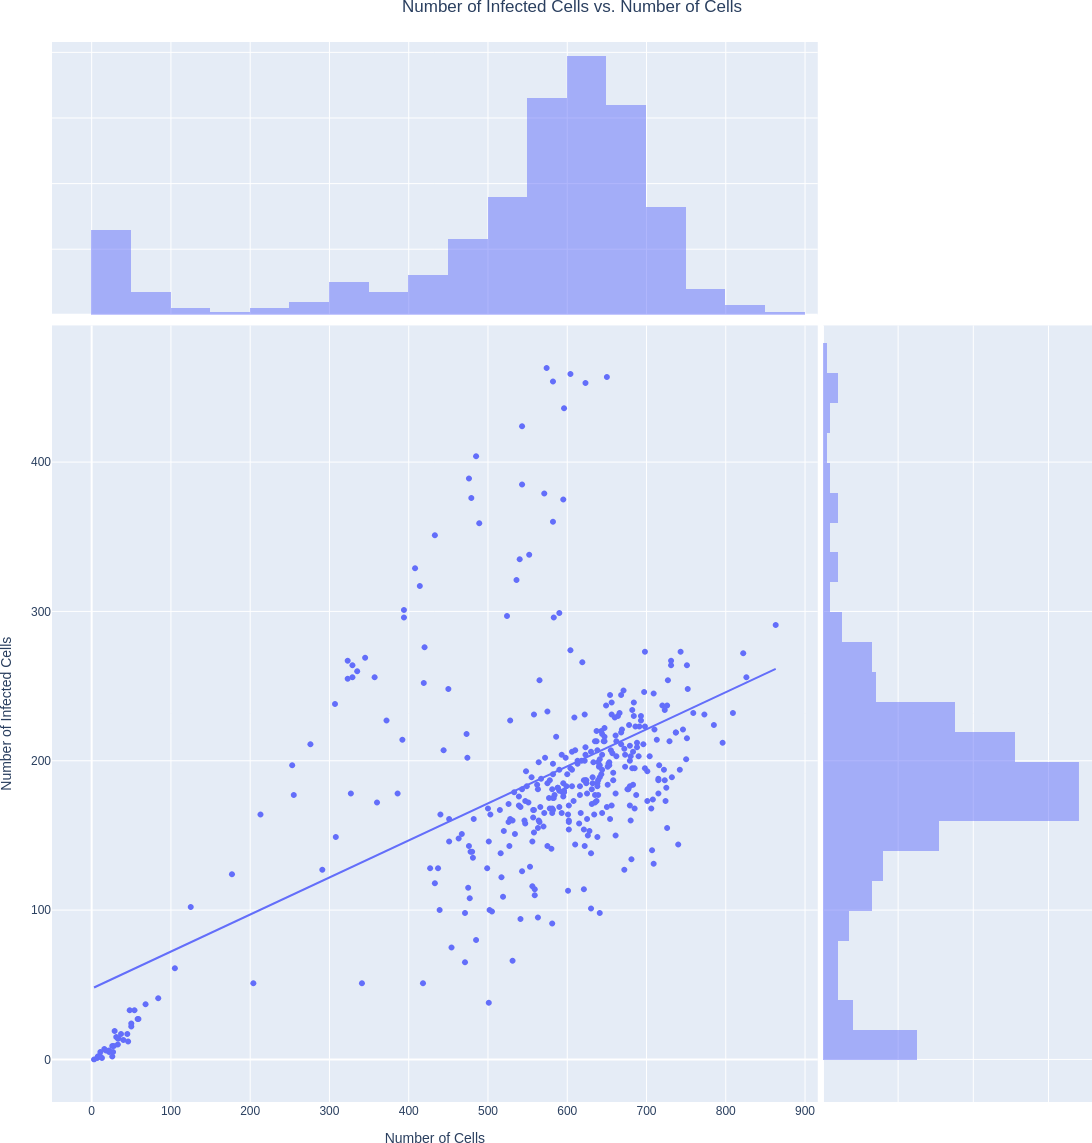
\includegraphics[width=0.7\textwidth, height=0.5\textwidth]{images/example_scatter.png}
    \caption{Exemplo de gráfico de dispersão interativo da placa de 384 poços.}
    \label{fig:scatter}
  \end{figure}

\end{itemize}

\section{Ajustando o pipeline \texttt{parasitecolocalization.cppipe}}

\section{Glossário}

Here is an \ac{Ex} of acronym usage.

\begin{acronym} \itemsep=-8pt
  \acro{Ex}[Ex]{Example}
\end{acronym}

\printbibliography

% \appendix

% \break \section{Supplementary Information}

% \renewcommand{\thefigure}{S\arabic{figure}}
% \setcounter{figure}{0}
% \renewcommand{\thetable}{S\arabic{table}}
% \setcounter{table}{0}

% \begin{table}[H]
%     \begin{center}
%         \begin{tabular}{|c|c|}
%             \hline
%             a & b \\\hline
%             c & d \\\hline
%         \end{tabular}
%     \end{center}
%     \caption[Shorter table caption]{Table caption caption caption caption
%         caption caption caption caption caption caption caption caption caption
%         caption caption caption caption caption caption caption caption caption
%         caption caption.}
%     \label{t:label0}
% \end{table}

% \begin{figure}[H]
% \centerline{
\includegraphics[scale=0.2]{lnbio-cnpem-logo.png}}
% \caption[Shorter figure caption]{Figure Caption caption caption caption
%   caption caption caption caption caption caption caption caption caption
%   caption caption caption caption caption caption caption caption caption
%   caption caption.}
% \label{f:label1}
% \end{figure}

\end{document}
